\title{Writing an Op-Ed %\thanks{}
}
\author[Marc Los Huertos]{Marc Los Huertos}
\date{}  % if the \date{} command is left out, the current date will be used

\begin{document}

\maketitle
\section{Rationale}

Communication is one of the key outcomes of an educated person. And in environmental issues, communication is critical to developing ways to engage and address a range of environmental issue. The Op-Ed is one of many powerful genres available to citizens to express criticism, make suggestions, or praise efforts to improve our society. 

\subsection{Learning Objectives}

This assignment is based on the EA learning outcome for writing and communicating: 

\begin{itemize}
	\item Understand the real-world processes and implications of environmental problem-solving and decision making.
	\item Speak and write clearly and persuasively.
\end{itemize}

\section{What is an Op-Ed?}

An op-ed, originally short for ``opposite the editorial page'', is an essay usually published by newspapers and magazines to expresses the opinions of a named author usually not affiliated with the publication's editorial board. Op-eds are different from both editorials, which are opinion pieces written by editorial board members, while letters to the editor are opinion pieces submitted by readers.

Most newspapers publish an opinion editorial page next to the editorial page. The newspaper's staff, syndicated columnists, or national and community opinion leaders often write the articles. However, the editors of most newspapers welcome the opinions of local citizens and leaders to add another dimension to their publication.

\subsection{Characteristics of a Op-Ed}

\begin{enumerate}
	\item Introduction, body and conclusion like other news stories
	\item An objective explanation of the issue, especially complex issues
	\item A timely news angle
	\item Opinions from the opposing viewpoint that refute directly the same issues the writer addresses
	\item The opinions of the writer delivered in a professional manner. Good editorials engage issues, not personalities and refrain from name-calling or other petty tactics of persuasion.
	\item Alternative solutions to the problem or issue being criticized. Anyone can gripe about a problem, but a good editorial should take a pro-active approach to making the situation better by using constructive criticism and giving solutions.
	\item A solid and concise conclusion that powerfully summarizes the writer's opinion. Give it some punch.
\end{enumerate}


\section{Types of Op-Eds}

\begin{description}
	\item[Explain or interpret:] Editors often use these editorials to explain the way the newspaper covered a sensitive or controversial subject. School newspapers may explain new school rules or a particular student-body effort like a food drive.
	\item[Criticize:] These editorials constructively criticize actions, decisions or situations while providing solutions to the problem identified. Immediate purpose is to get readers to see the problem, not the solution.
	\item[Persuade:] Editorials of persuasion aim to immediately see the solution, not the problem. From the first paragraph, readers will be encouraged to take a specific, positive action. Political endorsements are good examples of editorials of persuasion.
	\item[Praise:] These editorials commend people and organizations for something done well. They are not as common as the other three.
\end{description}
 

\section{Writing an Opinion Piece}
Give a concise, but thorough, background on the issue. Remember, the majority of people reading the story may not have an understanding of the issue. Give a thoughtful, yet brief, background on the issue before venturing into more details of the campaign.

Strengthen your message by citing national or international trends that show support for your thesis. Some factors  that influence public option on environmental issues include: a strong economy, the bipartisan support for the issue, the strength and diversity of the constituency, and the broad range of social benefits that might be gained.

Localize the story. Although environmental issues might be very broad and touches many lives across the USA or world, the readers for your opinion editorial will want to know how your thesis affects their community. Provide the audience with specific, well-known examples of how the successful implementation of your thesis can benefit the community in the future.


Although most newspapers keep an open mind in determining the content of their opinion editorials, some newspapers will be more inclined to publish an opinion piece on a subset of topics. Thus, it is important to research the newspaper in advance to appreciate the type of editorials it publishes, as well as what issues are covered in publication as a whole. Remember that a newspaper will not publish a story unless the editorial board feels it represents a unique or different perspective.

\subsection{Choose your topic wisely}

For maximum impact, choose an issue that has been making the headlines recently. For instance, if the Presidential elections are around the corner, focus on a particular topic with political implications. Additionally, be very specific about the issue you wish to focus on. You might have a lot to say about a dozen issues, but save your knowledge for later. Narrow down your area of interest with as much precision as is possible. This is a great opportunity to practice writing less and saying more!

\subsection{Declare your agenda outright}

An editorial without an unequivocal opinion is bound to fall flat on its face. Right at the very beginning, define your agenda in clear terms. Make sure that you state your opinion or thesis coherently. Remember those research papers and thesis statements you wrote in college. It's time to refresh your memory and concentrate on thesis statement writing skills. This course on how to write a thesis should help you immensely. The essential structure of a thesis statement in an editorial remains the same, only the language is more informal and journalistic.

\subsection{Build your argument}
A good editorial expresses your point of view while a great one manages to persuade others to join your camp. To persuade people, you need a sound argument based on facts and analogies, not vitriol and diatribe. Once you have stated your thesis, acknowledge contradictory opinions and explain why you disagree with them. Use facts, statistics, quotations and theoretical explanations for criticizing your opponents' views and cite your sources. Rejecting them outright without any explanation screams of cowardice and unprofessional ethics. Using external sources without citing them leaves you vulnerable to accusations that you made up the data or using the data inappropriately. 

To build a foolproof argument, you will need to achieve a balance between content and style. Not only will you need substantial data, you will also need to structure it coherently. Take this course to learn the basics of writing with writing with precision and clarity.


\subsection{Strengthen your argument with analogies}
Nothing disarms your opponents better than cultural, social or political analogies. For instance, if you are writing about a controversial issue like secret surveillance, look for similar instances in other countries and how they tackled the problem. You can use such an analogy to your benefit by highlighting both the similarities and the differences. This will also be a good time to speak about the ultimate consequences of a policy/law if appropriate action is not taken by concerned agencies.

\subsection{Provide possible solutions}
So, you have made a case for your views and demolished your opponents' claims. The journey doesn't end here. An editorial is primarily meant to indulge in constructive criticism i.e. even though it critiques one point of view, it must be able to provide a possible alternative. Say, your editorial attacked the efficacy of steps taken by the government to curb domestic violence in a particular region, conclude your piece by discussing other viable options. Once again, build an argument and talk about why these proposed steps are better than the ones already in place. Don't mistake an editorial for an opportunity to indulge in mindless criticism; instead, use it to offer a better vision for the future.

\section{Structuring your Op-Ed}

\subsection{Lead with an Objective Explanation of the Issue/Controversy}

\begin{enumerate}
	\item Include the five W's  (Who, what, where, when, and why) and the H (How). 

\paragraph{For example}

Members of Congress, in effort to reduce the budget, are looking to cut funding from public television. Hearings were held\ldots

	\item Pull in facts and quotations from the sources which are relevant.
	\item Additional research may be necessary.
\end{enumerate}

\subsection{Present Your opposition first} 

As the writer you disagree with these viewpoints. Identify specific people you oppose or disagree. 

\paragraph{For example} Republicans feel that these cuts are necessary; other cable stations can pick them; only the rich watch public television.

\begin{itemize*}
	\item Use facts and quotations to state objectively their opinions.

	\item Give a strong position of the opposition. You gain nothing in refuting a weak position.
\end{itemize*}
 
\subsection{Attempt to directly refute to the opposition's beliefs}

\begin{itemize*}
\item You can begin your article with transition that links to the objection.\sidenote{Remember, ``refute is a success term.  It is hard to refute a claim, and so real refutations are hard to come by. It is thus inappropriate to say (things like), `I refute your argument.' It is generally better to speak in terms of objections, which can be powerful and important even when (as is often the case) they do not constitute refutations.''--Ann Davis, ``Writing Papers Fall 2015''.}

\paragraph{For example} Republicans believe public television is a ``sandbox for the rich.'' However, statistics show most people who watch public television make less than \$40,000 per year.

\begin{marginfigure}
	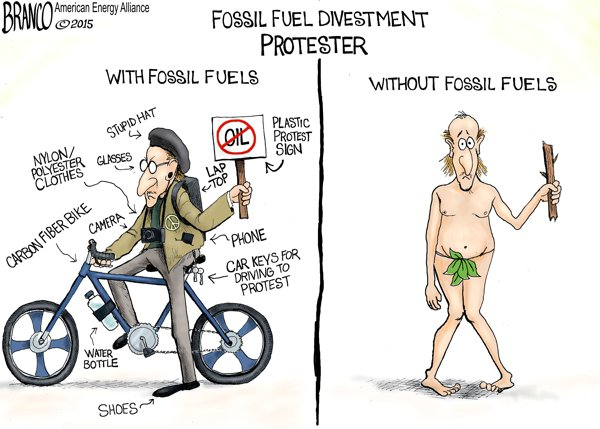
\includegraphics{Divestment-600-AEA-1.jpg}
	\caption{Take care to avoid the pitfalls of other's opinions. Try to cutoff counter arguments before they can ruin your arguments.}
	\label{fig:Divestment-600-AEA-1}
\end{marginfigure}


	\item Pull in other facts and quotations from people who support your position.
	\item Concede a valid point of the opposition which will make you appear rational, one who has considered all the options.
	
\paragraph{For example} Fiscal times are tough, and we can cut some of the funding for the arts; however, \ldots
\end{itemize*}

\subsection{Give additional, original reasons or analogies}

\begin{itemize*}
	\item In defense of your position, give reasons from strong to strongest order. 
	
\paragraph{For example} Taking money away from public television is robbing children of their education\ldots

	\item Use a literary or cultural allusion that lends to your credibility and perceived intelligence 
	
\paragraph{For example} We should render unto Caesar that which belongs to him\ldots
\end{itemize*}

\subsection{Conclude with a provocative statement or question}

\begin{itemize*}
	\item Give solutions to the problem or challenge the reader to be informed.
	
	\paragraph{For example} Congress should look to where real wastes exist --- perhaps in defense and entitlements --- to find ways to save money. Digging into public television's pocket hurts us all.
	
	\item A quotation can be effective, especially if from a respected source

	\item A rhetorical question can be an effective endpoint as well.
	
	\paragraph{For example} If the government doesn't defend the interests of children, who will?
\end{itemize*}



\section{Grading}

You will be grading for the following criteria with a goal of meeting the first standard for each:

\subsection{Communication}

Define a compelling and timely problem in your own words. 

Standards

\begin{enumerate*}
	\item Identifies the problem that demonstrates the topic is both compelling and timely with numerous supporting details and examples which are organized logically and coherently.		
	\item Identifies the problem with some supporting details and examples in an organized manner.	
	\item Identifies the problem with few details or examples in a somewhat organized manner.	
	\item Identifies the problem poorly with few or no details or states the main idea or problem verbatim from other sources.
	\item Does not identify problem.
\end{enumerate*}

\subsection{Analysis}

Present the opposition's argument with integrity and develop reasonable objections.

\begin{enumerate*}
	\item Uses specific inductive or deductive reasoning to make inferences regarding premises; addresses implications and consequences; identifies facts and relevant information correctly.	
	\item Uses logical reasoning to make inferences regarding solutions; addresses implications and consequences; Identifies facts and relevant information correctly.		
	\item Uses superficial reasoning to make inferences regarding solutions; Shows some confusion regarding facts, opinions, and relevant, evidence, data, or information.	
	\item Makes unexplained, unsupported, or unreasonable inferences regarding solutions; makes multiple errors in distinguishing fact from fiction or in selecting relevant evidence. 	
	\item Does not analyze multiple solutions.
\end{enumerate*}


\subsection{Problem Solving}
Select and defend your chosen solution.	
\begin{enumerate*}
	\item Thoroughly identifies and addresses key aspects of the problem and insightfully uses facts and relevant evidence from analysis to support and defend potentially valid solutions.	
	\item Identifies and addresses key aspects of the problem and uses facts and relevant evidence from analysis to develop potentially valid conclusions or solutions.	Identifies and addresses some aspects of the problem;  develops possible conclusions or solutions using some inappropriate opinions and irrelevant information from analysis. 	
	\item Identifies and addresses only one aspect of the problem but develops untestable hypothesis; or develops invalid conclusions or solutions based on opinion or irrelevant information.	
	\item Does not select and defend a solution.
\end{enumerate*}

\subsection{Evaluation}

Identify weaknesses in your chosen solution.	

\begin{enumerate*}
	\item Insightfully interprets data or information; identifies obvious as well as hidden assumptions, establishes credibility of sources on points other than authority alone, avoids fallacies in reasoning; distinguishes appropriate arguments from extraneous elements; provides sufficient logical support. 	
	\item Accurately interprets data or information;
identifies obvious assumptions, establishes credibility of sources on points other than authority alone, avoids fallacies in reasoning; distinguishes appropriate arguments from extraneous elements; provides sufficient logical support.	
	\item Makes some errors in data or information interpretation; makes arguments using weak evidence; provides superficial support for conclusions or solutions.	Interprets data or information incorrectly; 
	\item Supports conclusions or solutions without evidence or logic; uses data, information, or evidence skewed by invalid assumptions; uses poor sources of information; uses fallacious arguments.	
	\item Does not evaluate data, information, or evidence related to chosen solution. 
\end{enumerate*}

\subsection{Synthesis}

Suggest ways to improve/strengthen your chosen solution.

\begin{enumerate*}
	\item Insightfully relates concepts and ideas from multiple sources; uses new information to enhance chosen solution; recognizes missing information; correctly identifies potential effects of new information.	
	\item Accurately relates concepts and ideas from multiple sources; uses new information to enhance chosen solution; correctly identifies potential effects of new information.	
	\item Inaccurately or incompletely relates concepts and ideas from multiple sources; shallow determination of effect of new information on chosen solution.	
	\item Poorly integrates information from more than one source to support chosen solution; Incorrectly predicts the effect of new information on chosen solution.	
	\item Does not identify new information for chosen solution.	
\end{enumerate*}

\section{Grading}

The Op-Ed will be graded using the ``Op-Ed and Memo Grading Matrix'' found on \texttt{Sakai}.

